\section{Case study: gl-matrix}\label{case-study-gl-matrix}

\href{http://glmatrix.net}{Home}

glMatrix is designed to perform vector and matrix operations stupidly
fast! The latest version uses WebPack to manage the modules.

\subsection{APIs}\label{apis}

Exposed interfaces: \texttt{glMatrix}, \texttt{mat2}, \texttt{mat2d},
\texttt{mat3}, \texttt{mat4}, \texttt{quat}, \texttt{vec2},
\texttt{vec3}, \texttt{vec4}

\subsubsection{\texorpdfstring{\href{http://glmatrix.net/docs/2.2.0/symbols/glMatrix.html}{Common
utilities}}{Common utilities}}\label{common-utilities}

\begin{figure}[htbp]
\centering
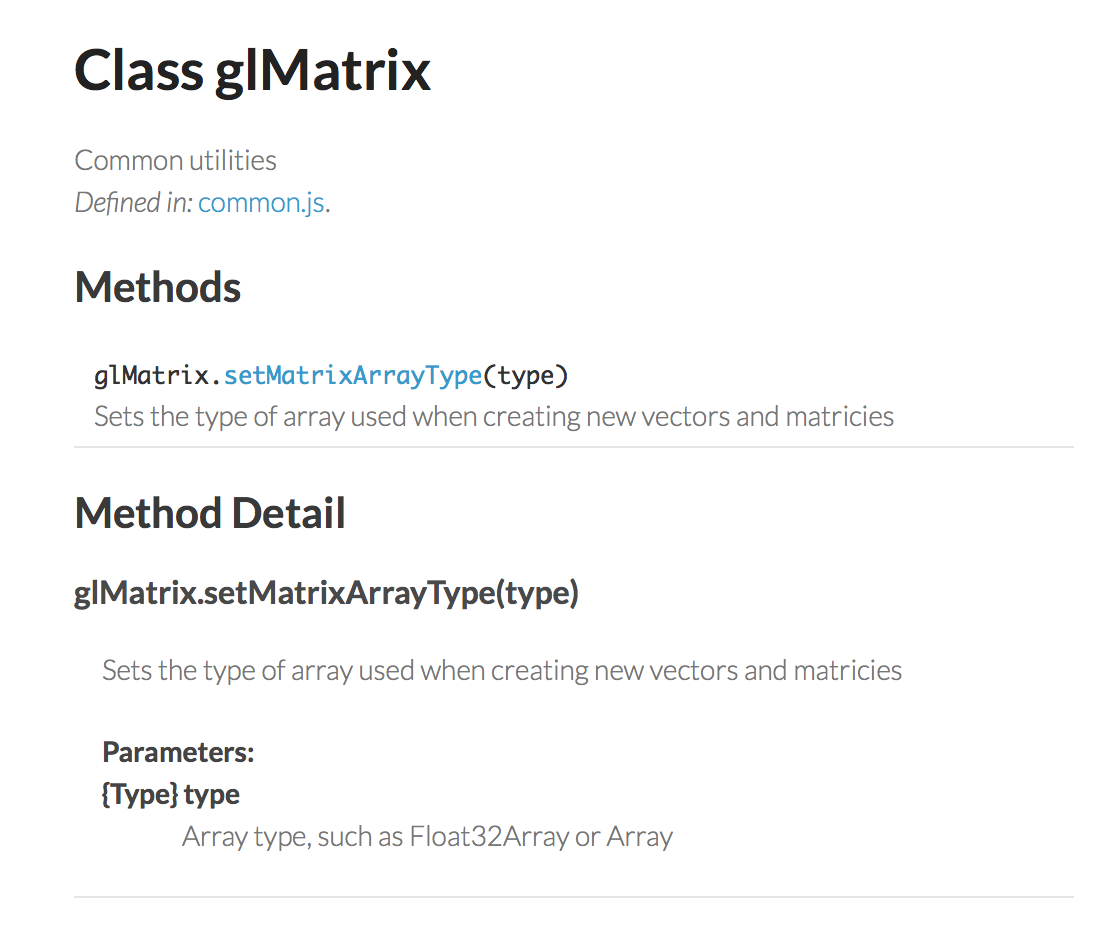
\includegraphics{gl-matrix.png}
\caption{}
\end{figure}

\subsubsection{\texorpdfstring{\href{http://glmatrix.net/docs/2.2.0/symbols/mat3.html}{3x3
Matrix}}{3x3 Matrix}}\label{x3-matrix}

\begin{figure}[htbp]
\centering
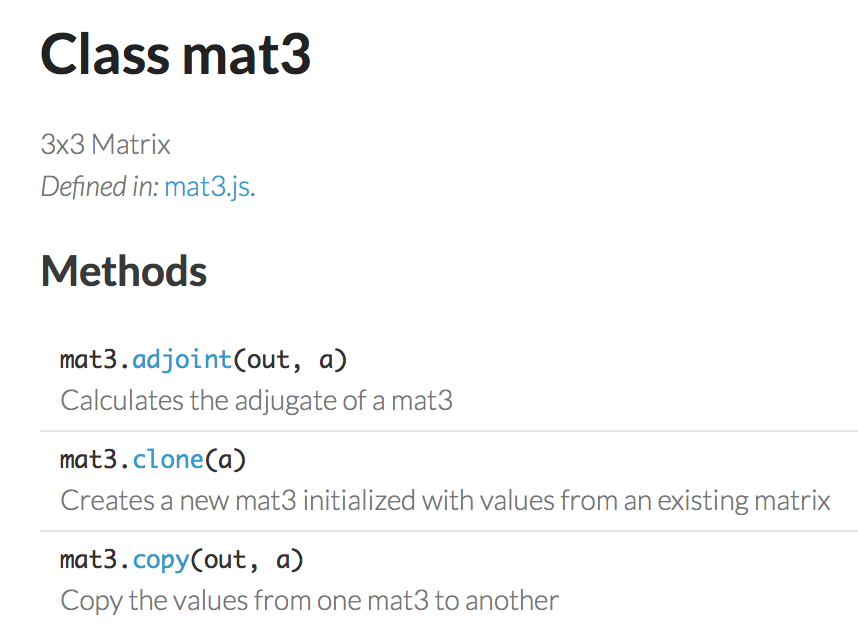
\includegraphics{mat3.png}
\caption{}
\end{figure}

\begin{figure}[htbp]
\centering
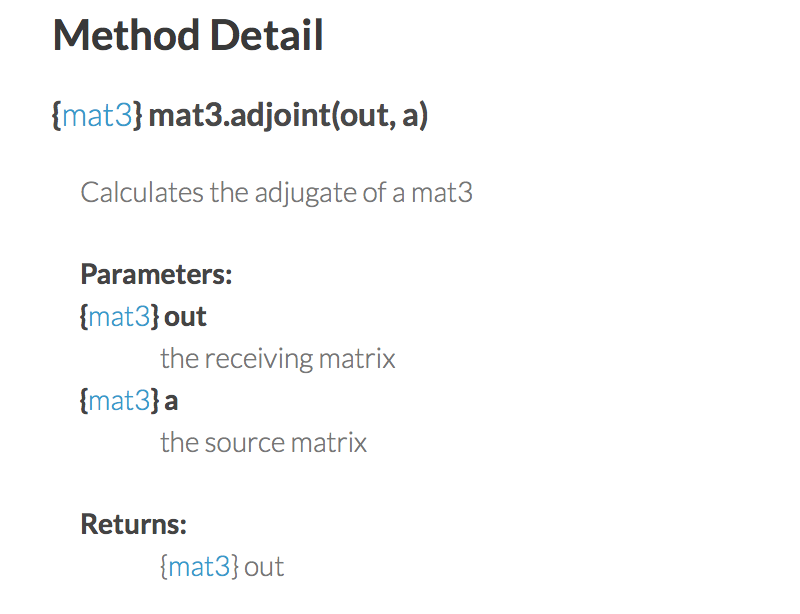
\includegraphics{mat3-adjoint.png}
\caption{}
\end{figure}

\subsection{Library structure}\label{library-structure}

\begin{itemize}
\tightlist
\item
  \texttt{glMatrix}: Common utilities, including config constants,
  compatibility detection, and things like \texttt{setMatrixArrayType}.
\item
  \texttt{mat3} etc: Represent one type of data and the related
  operations.

  \begin{itemize}
  \tightlist
  \item
    Constructors: \texttt{create}, \texttt{clone}, \texttt{copy}
  \item
    Computations: \texttt{identity}, \texttt{transpose}
  \item
    Conversions: \texttt{fromMat4}
  \end{itemize}
\end{itemize}

\subsection{Possible problems}\label{possible-problems}

\begin{enumerate}
\def\labelenumi{\arabic{enumi}.}
\tightlist
\item
  \textbf{Hard to maintain}: Even such a simple library is over 6000
  lines of JS; and the author suggested a ``sorry'' for breaking the
  APIs from 1.0 to 2.0.
\item
  \textbf{Type Unsafe}: Concretely, it is easy to pass a \texttt{vec3}
  to where a \texttt{vec4} is expected. And since here is no type
  checking, so you won't get any explicit warning.
\end{enumerate}
